% !TEX root = ../literature.tex
\subsection{Public space as a challenge for CDINUI}
Different field of studies have long held the view that the physical and social dynamics of public space play a central role in the formation of publics and public culture. Car et al, argued \emph{"when public spaces are successful […] they will increase opportunities to participate in communal activity. This fellowship in the open nurtures the growth of public life, which is stunted by the social isolation."} \cite{carr:1992}. For Computer Science this view was embraced with the new opportunities presented by the technological possibility to include the public space inside the ecology of a computer system. As such research investigating how public space can affect interaction with the system and vice versa spanned.\\

In historical perspective Brignull and Rogers work\cite{Brignull:2003} is the first that investigates interaction flow in the context of public space for large displays. They observe that even though large displays are increasingly placed in public places, to support community and social activities, people are reluctant to use them. They point out that the main reason, for existing resistance by the public to participate, is the prominence of the affective aspect of the  user experience - feelings of social embarrassment. In order to understand this phenomenon they create a conceptual framework for analyzing public interaction. Their framework consist of three different spaces (1) Space A peripheral awareness of displays - people are engage in unrelated activities (2) Space B focal awareness - - people are engage in associated activities (3) Space C direct interaction - people engage in interaction with the display. They point out \emph{it appears that the key bottlenecks occurs in public interaction when people have to make transitions between different activity spaces}. They conclude  it is key for public interaction to be able seamlessly and comfortably to transition between onlooker and participant and one way to do that is to encourage people to cross the thresholds from peripheral awareness to focal awareness, without becoming self-conscious.\\

While Brignull and Rogers work focuses on interaction with Large Displays, Cheung et al.  extends that to \emph{Interaction Barriers in Large Public Displays Using Personal Device.} \cite{Cheung:2014}. They focus on interaction process comprised of personal devices (capturing unique traits such as privacy and novel interaction mechanisms), and a large display (which is used as a shared display, and a direct input alternative, if supported) and list in partial order the usage barriers, for engaging a passerby, while clustering them in three groups (1) Attract - how can we combat display blindness (notice the display), interaction blindness (be aware we can interact with the display), and cross-device blindness (be aware we can use personal devices as a mean of interaction); (2) Interact - how can we combat complex interaction (easily understand how to make use of large display and personal device), social inhibition (do not feel social embarrassment),  and how can we opt-in/out (engage or withdraw from the system); (3) Manage - how can we maintain and communicate the connection between the large display and personal device (connecting, explicit disconnecting, implicit disconnecting), how can we recover from interrupting states (eg. Phonecall). After identifying the barriers to cross - device interaction \ref{fig:111} they model the interaction process as a series of states \ref{fig:222} stating that ideally a passerby will proceed through each state and engage the system. They conclude that each barrier in their design framework must be addressed in order for the users to be enticed to interact with the system.


\begin{figure}[H]
	\centering
	\subfloat[]{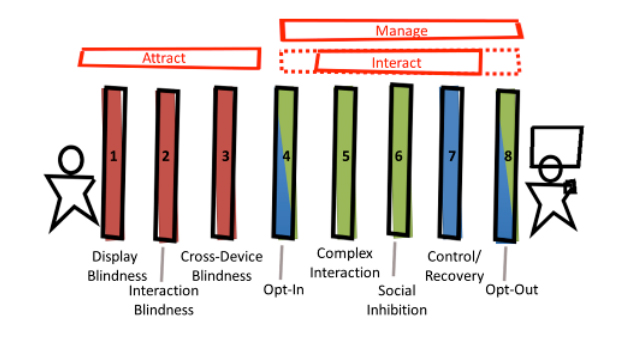
\includegraphics[width = 0.5\columnwidth , height = 2cm ]{images/111.jpg}\label{fig:111}} 
	\subfloat[]{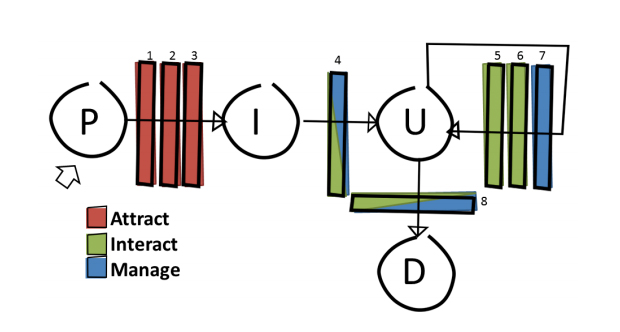
\includegraphics[width = 0.5\columnwidth , height = 2cm ]{images/222.jpg}\label{fig:222}}
	\caption{
		adopted from Cheung et al. \protect\cite{Cheung:2014}.
		\protect\subref{fig:111} cross-device interaction barriers for intercating with large displas and handheld device
		\protect\subref{fig:222} States  of interaction and barriers encountered.(P:Passing, I:Interested, U:Using, D:Done).
		}
	\label{fig:Cheung et al. ideas}
\end{figure}
\todo{Figgure, adopted - add cite. Prefer rephrasing}
